% !Mode:: "TeX:UTF-8"
\documentclass[13pt,fontset=mac]{ctexbeamer}
\usepackage[utf8]{inputenc}


\usepackage{amsmath,amssymb,amsthm}             % AMS Math
%\usepackage[T1]{fontenc}
\usepackage{graphicx}
\usepackage{epstopdf}
\usepackage{tikz}
\linespread{1.3}

\usepackage{mathrsfs}  %花写字母
 

%%%=== theme ===%%%
% \usetheme{Warsaw}
%\usetheme{Copenhagen}
%\usetheme{Singapore}
\usetheme{Madrid}
%\usefonttheme{professionalfonts}
%\usefonttheme{serif}
% \usefonttheme{structureitalicserif}
%%\useinnertheme{rounded}
%%\useinnertheme{inmargin}
\useinnertheme{circles}
%\useoutertheme{miniframes}
\setbeamertemplate{navigation symbols}{}
\setbeamertemplate{footline}[page number]



%\usepackage[fontset=mac]{ctex}
%\usepackage{ctex}
% \usepackage{CJK,CJKnumb,CJKulem}
%\usepackage{minitoc}


\setbeamertemplate{theorems}[numbered]
\newtheorem{thm}{定理}
\newtheorem{lem}{引理}
\newtheorem{exa}{例}
\newtheorem*{theo}{定理}
\newtheorem*{conj}{猜想}
\newtheorem*{defi}{定义}
\newtheorem*{coro}{推论}
\newtheorem*{ex}{练习}
\newtheorem*{rem}{注}
\newtheorem*{prop}{性质}
\newtheorem*{qst}{问题}

\def\qed{\nopagebreak\hfill{\rule{4pt}{7pt}}\medbreak}
\def\pf{{\bf 证明~~ }}
\def\sol{{\bf 解~~ }}



\def\R{\mathbb{R}}
\def\Rn{\mathbb{R}^n}
\def\A{\mathscr{A}}
\def\B{\mathscr{B}}
\def\D{\mathscr{D}}
\def\E{\mathscr{E}}
\def\O{\mathscr{O}}

\def\rank{\operatorname{rank}}
\def\dim{\operatorname{dim}}
\def\0{\mathbf{0}}
\def\a{\alpha}
\def\b{\beta}
\def\r{\gamma}

\usepackage{color}
\definecolor{linkcol}{rgb}{0,0,0.4}
\definecolor{citecol}{rgb}{0.5,0,0}

\definecolor{blue}{rgb}{0,0.08,1}
\newcommand{\blue}{\textcolor{blue}}

  \usepackage{graphicx}
  \DeclareGraphicsExtensions{.eps}
%   \usepackage[a4paper,pagebackref,hyperindex=true,pdfnewwindow=true]{hyperref}


\begin{document}



\title[]{高等代数}
\author[]{{\large 张彪} }
\institute[]{{\normalsize
		天津师范大学\\[6pt]
		zhang@tjnu.edu.cn}}

\date{}



\AtBeginSection[]
{
\begin{frame}
	\frametitle{Outline}
	\tableofcontents[currentsection]
\end{frame}
}



\begin{frame}
\maketitle
\end{frame}

\begin{frame}
\frametitle{\textcolor{orange}{Outline}}
\tableofcontents
\end{frame}





\section{引言}



	


\begin{frame}

\begin{columns}[c]  %开始进入分栏环境,居中设置
	
	\column{6cm}
\begin{leftline}
	{\Large  宇宙之大,粒子之微,} \\[8pt]
	
	{ \Large 火箭之速,化工之巧,}\\[8pt]
	
	{ \Large 地球之变,生物之评,}\\[8pt]
	
	{ \Large 日用之繁,无处不用数学。}
\end{leftline}


%\rightline{ {\Large 一华罗庚 \qquad \qquad\qquad}}
	\column{5cm} 
	\begin{figure}[p]
		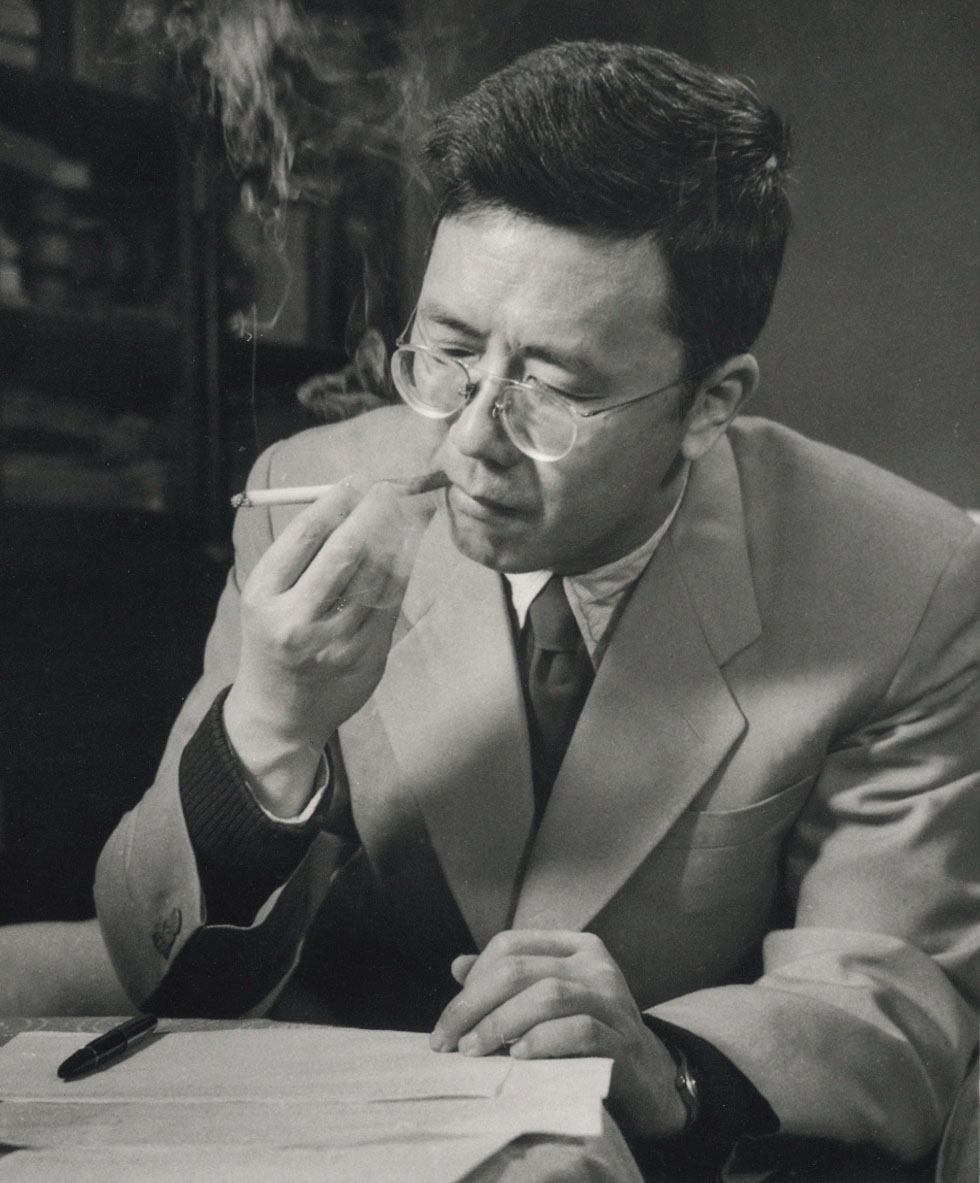
\includegraphics[scale=0.5]{hua.jpg}
		\caption{华罗庚 (1910--1985)}
	\end{figure}
	
\end{columns}

\end{frame}


\begin{frame}
	
	\begin{columns}[c]  %开始进入分栏环境,居中设置
		
		\column{6cm}
		\begin{figure}[p]
	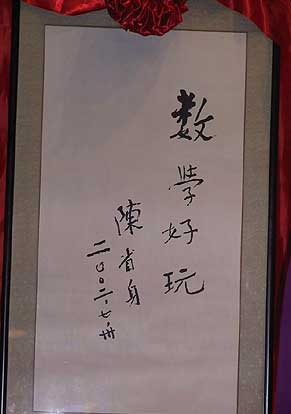
\includegraphics[scale=0.4]{数学好玩.jpg}
\end{figure}

		\column{5cm} 
		\begin{figure}[p]
			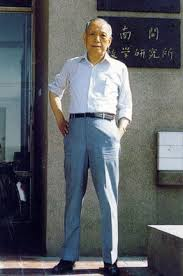
\includegraphics[scale=0.5]{chern.jpeg}
					\caption{陈省身 (1911-2004)}
		\end{figure}
	\end{columns}
\vspace{6pt}
			2002年8月在北京举行国际数学家大会(ICM2002)期间,91岁高龄的数学大师陈省身先生为少年儿童题词,写下了“数学好玩”4个大字。
\end{frame}




\begin{frame}
	自然科学的发展往往是在推翻或修正旧的理论基础上建立新理论的大厦。
	\begin{itemize}
		\item 哥白尼的地动说推翻了统治人们思想1500年的托勒密地心说
		\item 伽利略的比萨斜塔落体实验否定了亚里士多德的错误想象
		\item 爱因斯坦的相对论则是对牛顿运动定律的修正。
	\end{itemize}
\end{frame}



		\begin{frame}
	\begin{itemize}
		\item 然而,作为自然科学的共同语言,数学的独特之处在于它不需要被订正,新的数学理论只是为旧的建筑添砖加瓦,而无须连根拔起。
		\item 在数学里,已经证明为真的的命题永远为真。比如勾股定理(毕达哥拉斯定理)。
		\item 欧氏几何源于公元前3世纪。古希腊数学家欧几里德把人们公认的一些几何知识作为定义和公理(公设),在此基础上研究图形的性质,推导出一系列定理,组成演绎体系,写出《几何原本》,形成了欧氏几何。
		\item 美国卓越的犹太人科普作家阿西莫夫所说:“托勒密也许对天体系统给出了错误的描绘,但他为了计算而发展处的三角系统永远保持正确。”
	\end{itemize}
\end{frame}

\begin{frame}
	代数学起源于人类对于数的理解
	
	\vspace{6pt}
	
	代数学习的几个阶段
	\begin{itemize}
		\item 算~~术 :自然数、正分数的四则运算(小学)
		\item 初等代数:有理数、无理数、复数、解方程(中学)
		\item 高等代数:多项式、线性代数(大一)
		\item 近世代数:群、环、域(大二)
		\item $\cdots \cdots\cdots$
	\end{itemize}
\end{frame}

%
%\begin{frame}
%大约在 1637 年,法国数学家 Fermat 断言,
%\begin{conj}
%	对于大于 2 的整数 $n$,三个未知量 $x, y, z$ 的代数方程 $x^{n}+y^{n}=z^{n}$ 没有正整数解. 
%\end{conj}
%\pause
%
%%这个问题中,只牵涉到正整数的加法与乘 法(乘方)运算,可说是再简单不过了,具有初中一年级代数知识的人 都能看明白.
%
%%但是
%它历经 350 余年,无数第一流的数学家为之纹尽脑汁, 才于 1994 年被 Princeton 大学的数学家 Wiles 使用现代最深奥 的数学理论得出解答. 
%
%\end{frame}
%
%
%
%\begin{frame}
%\begin{itemize}
%\item 从生产实践和自然科学理论中,自然地产生了\alert{求解代数方
%程}的问题,它就是代数学的经典课题.
%\item 
%例如,根据牛顿第二运动定律, 物体所受的力 F,它的质量 $m$ 和产生的加速度 $a$ 之间存在关系 $F=$ ma. 
%如果已知物体的质量 $m$ 和所受的力 $F$,求加速度 $a,$ 这就是\alert{一元 一次方程}的求解问题.
%\item  又比如,一个以初速 $v_{0}$ 在水平面上作匀加速 运动的物体,它的加速度 a,运动时间 $t$ 和移动的距离 S 满足
%\[
%S=v_{0} t+\frac{1}{2} a t^{2}
%\]
%如果已知 $S, v_{0}, a,$ 求运动时间 $t,$ 这就是求\alert{一元二次方程}的根.
%\end{itemize}
%
%
% 
%
%\end{frame} 
%
%
%\begin{frame}
%\begin{itemize}
%\item 数学 史表明,早在中世纪人们就已经找到解一元一次、二次代数方程的一 般方法. 
%\item 到欧洲的文艺复兴时代,又找到\alert{一元三次、四次方程}的求根 公式. 
%\item 但是随后数学家们就碰到难题了. 在数百年时间内,他们苦苦 寻求五次以上代数方程的求根公式,却总是遭到失败. 
%\pause
%\item 直到 1832 年, 法国数学家 Galois 才找到了一个\alert{高次代数方程}有根式解(即用该方 程的系数经加、减、乘、除及开方运算表示它的全部根)的判别准则, 完满地解决了高次代数方程根的理论课题. 
%\end{itemize}
%\end{frame}
%
%
%\begin{frame}
%\begin{itemize}
%	\item
%	根据 Galois 的理论,五 次以上的一般代数方程没有求根公式. 
%
%	\item Galois 的工作中最值得注意 的是,他不是局限在数的四则运算的范围内考查问题. 
%
%	\item 他跳出这个圈 子,考查 $n$ 次方程的 $n$ 个根的某些\alert{置换}所组成的集合 $G,$ 规定 $G$ 内两 个置换的“乘积”是对根的集合逐次进行这两个置换. 
%
%	\item 他在一个 并非由数组成的集合 G 内定义了一种新的代数运算:\alert{乘法}(它完全 不同于数的乘法). 他发现这种乘法也具有与数的乘法相类似的某些 运算法则(例如满足结合律等等). 这个新的具有乘法运算的集合我 们现在把它称为该高次代数方程的 \alert{Galois 群}. 
%
%	\item Galois 证明:
%\begin{center}
%高次代 数方程有没有根式解取决于它的 Galois 群的结构. 
%\end{center}
%\end{itemize}
%\end{frame}
%
%\begin{frame}
%\begin{itemize}
%	\item 这样,人们的认 识发生了一个质的飞跃,那就是为了研讨数及其代数运算中所包含 的深刻规律,我们必须跳出数及其四则运算的框框,去研究一个更一 般的集合及其中应有的代数运算.
%
%	\item  这样 ,代数学发生了一个革命性的 变化:从研究代数方程的求根这一经典课题解脱出来,变成研究一 个一般的\alert{集合}(其元素可以完全抽象,没有具体内容),在其中存在一 种或若干种\alert{代数运算}(这种运算不同于数的四则运算,甚至可以是抽 象定义的),同时要求这些运算要满足一定的运算法则. 
%\end{itemize}
%\end{frame}



\begin{frame}{教材}
	教材
	
	\begin{itemize}
		\item 北京大学数学系几何与代数教研室代数小组, 高等代数(第5版), 高等教育出版社, 2019.
		
		
	\end{itemize}
	
	参考书目
		\begin{itemize}
		
		\item  王萼芳, 石生明, 高等代数辅导与习题解答(北大·第5版), 高等教育出版社, 2019.
		
		\item 徐仲等, 高等代数(北大第四版)导教导学导考, 西安:西北工业大学出版社, 2014.
		
	\end{itemize}

\end{frame}



\begin{frame}{Outline}
	
		\begin{columns}[c]  %开始进入分栏环境,居中设置
		
		\column{6cm}

\alert{第一学期}
\begin{itemize}
	\item[1]多项式
	\item[2] 行列式
	\item[3] 线性方程组
\end{itemize}

\alert{第二学期}
\begin{itemize}
	\item[4] 矩阵
	\item[5] 二次型
	\item[6] 线性空间
	\item[7] 线性变换
	\item[9] 欧几里得空间
\end{itemize}
		
		\column{5cm} 
		\begin{figure}[p]
			
\includegraphics[scale=0.5]{gaodai_code.png}
			\caption{课程网页}
		\end{figure}
	\end{columns}

\end{frame}




\section{充分必要条件}

\begin{frame}{充分条件和必要条件}
设A与B为两命题,
\begin{itemize}
	\item A的\alert{充分条件}是B
	
	如果B成立,那么A成立,即$A\Leftarrow B$(箭头表示能够推导出)
	
	\item A的\alert{必要条件}是B
	
	如果A成立,那么B成立,即$A\Rightarrow B$.
	
	\item A的\alert{充分必要条件}是B
	\begin{itemize}
		\item 充分性 $A\Leftarrow B$
		\item 必要性 $A\Rightarrow B$
	\end{itemize}
	
\end{itemize}


\end{frame}
\begin{frame}{当且仅当}
当且仅当(英文:If and only if, 或者:iff),在数学、哲学、逻辑学以及其他一些技术性领域中广泛使用,在英语中的对应标记为iff。

设A与B为两命题,在证明
\begin{center}
A当且仅当B
\end{center}
时,这相当于去同时证明陈述
\begin{itemize}
\item 如果A成立,那么B成立
\item 如果B成立,把么A成立
\end{itemize}


%另外,也可以证明“如果A成立,则B成立”和“如果A不成立,则B不成立”,后者作为对偶,等价于“如果B成立,则A成立”。

公认的其他同样说法还有
\begin{center}
B是A的充分必要条件(或称为充要条件).
\end{center}
%
%一般而言,当我们看到“A当且仅当B”,我们可以知道“如果A成立时,则B一定成立”、“如果B成立时,则A也一定成立”、“如果A不成立时,则B也一定不成立”、“如果B不成立时,则A也一定不成立”。
%
%当且仅当A(命题)成立时,B(命题)成立。
%
%也可表示成:B(命题)成立时,A(命题)成立 ;A(命题)成立时,B(命题)成立。即B(命题)等价于A(命题)。
%
%通俗一点来说,就是“在这些情况下,并且仅仅在这些情况下”。
注: 在定义中,``如果…那么…''的意思就是当且仅当。

比如书上两个多项式相等的定义。
\end{frame}



\section{数学归纳法}

\begin{frame}


如果你有一排很长的直立着的多米诺骨牌那么如果你可以确定:

第一张骨牌将要倒下. 

只要某一个骨牌倒了,与他相临的下一个骨牌也要倒. 

那么你就可以推断所有的的骨牌都将要倒. \\[15pt]
		
\includegraphics[scale=0.4]{gupai.jpg}
\end{frame}


\begin{frame}{第一数学归纳法}
第一数学归纳法可以概括为以下三步:
\begin{enumerate}
\item 归纳奠基:证明$n=1$时命题成立.
\item 归纳假设:假设$n=k$时命题成立.
\item 归纳递推:由归纳假设推出$n=k+1$时命题也成立.
\end{enumerate}


\end{frame}

\begin{frame}
\begin{exa}
证明对于任意自然数$n$,下面的公式都成立
\[
1+2+3+\cdots+n=\frac{n(n+1)}{2}.
\]
\end{exa}
%这是用于计算前 $n$ 个自然数之和的公式. 

\pf 
\begin{itemize}
\item 这个公式在 $n=1$ 时成立.  左边 = 1,右边 = 1(1+ 1) / 2 = 1. 

所以这个公式在 $n=1$ 时成立. 
\item 我们假设 $n=m$ 时公式成立,即
\[
1+2+\cdots+m=\frac{m(m+1)}{2}.
\]
\item 在上式等号两边分别加上 $m+1$ 得到
\[
1+2+\cdots+m+(m+1)=\frac{m(m+1)}{2}+(m+1) = \frac{(m+1)(m+2)}{2}.
\]
这就是 $n=m+1$ 时的等式. 

因此,对于任意自然数等式都成立. \qed
\end{itemize}
\end{frame}

\begin{frame}
\begin{exa}
对于任意自然数$n$证明$3^n−1$ 是 $2$ 的倍数.
\end{exa}
\pf 

\begin{itemize}
	\item  $3^0−1 = 1−1 = 0$是$ 2 $的倍数.  所以, 当 $n=0$ 时命题成立. 
	\item 我们假设 $n=k$ 时命题成立, 即 $3^{k}−1$ 是 $2$ 的倍数.
	\item 接下来证明$n=k+1$ 时命题也成立. 
	\begin{align*}
		3^{k+1}-1 & = 2 \cdot 3^{k}+(3^{k}-1 )
	\end{align*}
	$2 \cdot 3^{k}$是 $2$ 的倍数.
	由归纳假设,$3^{k}−1$ 是 $2$ 的倍数.
	又因为$2 \cdot 3^{k}$也是 $2$ 的倍数, 
	所以	$3^{k+1}-1$是 $2$ 的倍数.
	
	因此,对于任意自然数$n$,都有 $3^n−1$ 是 $2$ 的倍数.
	 \qed
\end{itemize}
\end{frame}

\begin{frame}
	\begin{exa}[思考题]
给定圆周上任意$n$个点,确定有$\binom{n}{2}:=\frac{n(n-1)}{2}$条弦划分的圆内的区域数$R_n$,这里假设任意三条弦在圆内不相交。
	\end{exa}




\end{frame}

\begin{frame}{第二数学归纳法}
有些命题用第一归纳法证明不大方便,可以用第二归纳法证
明. 

第二数学归纳法的证明步骤是:
\begin{enumerate}
\item 证明当 $n=1$时命题成立.
\item 假设$n\le k$ 时命题都成立.
\item 由归纳假设推出 $n=k+1$时命题也成立.
\end{enumerate}
\end{frame}






\section{连加号}

\begin{frame}
		\small{
	在数学中经常碰到若干个数连加的情况
	\begin{align}\label{eq:a_i}
		a_1+a_2+\cdots+a_n
	\end{align}
	为了简便起见,我们通常记成
	\begin{align}\label{eq:a_i_sum}
		\sum_{i=1}^{n}a_i
	\end{align}
	$\sum$称为\alert{连加号},而连加号上下的写法表示$i$的取值由$1$到$n$.
	
	例如
	\[1^2+2^2+\cdots+n^2=\sum_{i=1}^{n}i^2\]
	
	这里的 $i$ 称为\alert{求和指标}, 它只起一个辅助的作用.
	
	把 \eqref{eq:a_i_sum}还原成 \eqref{eq:a_i} 时,
	它是不出现的.譬如说, \eqref{eq:a_i}也可以记成
	$$
	\sum_{j=1}^{n} a_{j}
	$$
因之,只要不与连加号中出现的其它指标相混,用什么字母作为求和指标是
	任意的.}
\end{frame}




\section{整数的可除性理论}
\begin{frame}{整数的可除性理论}
%整数及其运算是大家熟悉的. 整数包括正整数,零及负整数.

%用 $\mathbb{N}$
%表示全体正整数组成的数集,而

用 $\mathbb{Z}$ 表示全体整数组成的数集.

%这一附录引导读者学习整数的可除性理论.这是学习高等代数以及其它 课程必须知道的数学知识. 我们列出了所有的结论,但没有证明.读者完全可 以仿照多项式理论中有关结论的论证补出这些证明.这是留给读者的绝好的
%练习

整数有加法, 减法和乘法等运算, 减法是加法的逆运算. 

%加法和乘法满足 下面的八条规律.
%以下用 $a, b, c, d, \ldots$ 表示任意整数.
%\begin{enumerate}
%\item 加法交换律: $a+b=b+a$
%\item 加法结合律: $(a+b)+c=a+(b+c)$
%\item $\mathbb{Z}$ 中有零元素 0,满足
%$a+0=0+a=a$
%\item 每个整数 $a $都有唯一的负元素 $- a$, 使得
%$a+(-a)=(-a)+a=0$
%\item 乘法交换律: $a \cdot b=b \cdot a$
%\item  乘法结合律: $(a \cdot b) \cdot c=a \cdot(b \cdot c)$
%\item 分配律 : $a \cdot(b+c)=a \cdot b+a \cdot c$
%\item 消去律: 如果 $a \cdot b=a \cdot c, a \neq 0,$ 则 $b=c$
%\end{enumerate}
%根据第 4 条, 减法可看成是加法的逆运算$a-b:=a+(-b)
%$
%\end{frame}
%
%
%\begin{frame}{整 数 的可除 性 理 论}
\begin{itemize}
\item 带余除法
\item 整除
\item 最大公因数
\item 辗转相除法
\item 互素
\item 素数
\item 因数分解定理
\item 最小公倍数
\end{itemize}
\end{frame}
\begin{frame}{带余除法}
在 $\mathbb{Z}$ 中不能作除法,但是有以下的\alert{带余除法}.  
\begin{thm}
对于任意两个整数 $a ,b,b\neq 0$,存在一对整数 $q, r$ 满足
\[
a=q \cdot b+r, \quad 0 \leqslant r<|b|
\]
而且满足这个条件的整数 $q, r$ 是唯一的. 
\end{thm}
\begin{defi}
\begin{itemize}
\item $q$ 称为b 除 $a$ 的\alert{商}, 
\item $r$ 称为 $b$ 除 $a$ 的\alert{余数}. 
\end{itemize}
\end{defi}
 
\end{frame}

\begin{frame}
\begin{defi}
	对于整数 $a ,b$,如果存在一个整数 $c$ 使得 $a=b c,$ 则称
\begin{itemize}
\item $b$ 是 $a$ 的\alert{因数}, 
\item $a$ 是 $b$ 的\alert{倍数}.
\end{itemize}
\end{defi}
\begin{rem}
在定义中我们并不要求 $b\neq0$. 
\end{rem}


\end{frame}

\begin{frame}

\begin{prop}
	当 $b\neq 0$ 时,$b$ 是 $a$ 的因数的充 分必要条件是 $b$ 除 $a$ 所得的余数为 $0$.
\end{prop}
因此 $b$ 是 $a$ 的因数, 也称 $b$ \alert{整除} $a,$ 记作$b | a$. 

关于整除,有以下一些性质:
\begin{prop}
\begin{enumerate}
\item 如果 $a|b, b| a,$ 则 $a=\pm b$
\item 如果 $a|b, b| c,$ 则 $a | c$
\item  如果 $a|b, a| c,$ 则对任意整数 $k, l$ 都有 $a | k b+l c$
\end{enumerate}
\end{prop}
\begin{rem}
\begin{itemize}
\item 如果 $a | b,$ 则有 $-a | b$ 及 $a |(-b),$ 因此以后我们只讨论\alert{非负整数}的\alert{非 负因数}和\alert{非负倍数},不再加以说明.

\item 根据定义,每个整数都是 0 的因数,但是 0 不是任何非零整数的因数.
\end{itemize}
\end{rem}

\end{frame}




\begin{frame}
\begin{defi}
如果 $a$ 既是 $b$ 的因数,又是 $c$ 的因数,则称 $a$ 是 $b$ 和 $c$ 的一个\alert{公因数}.
\end{defi}
公因数中最重要的是最大公因数.

\begin{defi}
设 $d$ 是 $a$ 和 $b$ 的一个公因数. 如果 $a, b $的任一个因数都是 $d$ 的
因数, 则称 $d$ 是 $a, b$ 的一个\alert{最大公因数}.
\end{defi}

\begin{rem}
	\begin{itemize}
\item 根据定义,如果 $d_{1}, d_{2}$ 都是 $a, b$ 的最大公因数,那么 $d_{1}\left|d_{2}, d_{2}\right| d_{1} .$ 从
而 $d_{1}=\pm d_{2} .$ 
按规定 $d_{1}, d_{2}$ 皆非负,故 $d_{1}=d_{2}$.

\item 当 $b | a$ 时, $b$ 是 $a$ 与 $b$ 的最大公因数.

\item 特别地当 $a=0$ 时, $b$ 是 $a$ 与 $b$ 的一 个最大公因数.
 
\item 当 $a, b$  不全为零时, $a,b$ 的最大公因数不为0,  这时我们规定:以$(a, b)$ 表示 $a, b$ 的正的最大公因数. 在这个规定下,$(a, b)$是唯一的. 
\end{itemize}
\end{rem}
\end{frame}

\begin{frame}{辗转相除法}

设 $b \neq 0,$ 即 $b>0 .$ 反复应用 带余除法. 
	\[
	\begin{array}{cc}
	a=q_{1} b+r_{1}, & 0<r_{1}<b \\
	b=q_{2} r_{1}+r_{2}, & 0<r_{2}<r_{1} \\
	\cdots  & \cdots  \\
	r_{k-2}=q_{k} r_{k-1}+r_{k}, & 0<r_{k}<r_{k-1} \\
	r_{k-1}=q_{k+1} r_{k}+0
	\end{array}
	\]
	直到出现余数为零而终止. 则有
	\[
	(a, b)=\left(b, r_{1}\right)=\left(r_{1}, r_{2}\right)=\cdots=\left(r_{k-1}, r_{k}\right)=r_{k}
	\]
	从上面的算法中还可以找到整数 $u, v$ 使得
	\[
	(a, b)=u a+v b
	\]
	这是最大公因数的重要性质.
\end{frame}


\begin{frame}
\begin{defi}
	如果整数 $a, b$ 的最大公因数等于 1,则称 $a, b$ \alert{互素} (亦称互质).
\end{defi}
例如,3 与5互素, 21 与 40 互素.

互素有以下一些重要性质:
\begin{enumerate}
\item $a ,b$ 互素的充分必要条件是存在整数 $u, v$ 使
\[
u a+v b=1
\]
\item 如果 $a | b c,$ 月 $(a, b)=1,$ 则 $a | c$.
\item 如果 $a|c, b| c$ 而且 $(a, b)=1,$ 则 $a b | c$
\item 如果 $(a, c)=1,(b, c)=1,$ 则 $(a b, c)=1$
\end{enumerate}
这些性质说明了互素的重要性. 
\end{frame}


 
 \begin{frame}
%最后介绍素数(亦称质数)的概念.  

%一个整数 $a(a>1)$ 至少有两个因数: 1 和 $a$ 本身. 不等于 1 和 $a$ 的因数 叫做 $a$ 的真因数.  

\begin{defi}
	$a$ 是一个大于 1 的整数.如果除去 1 和本身外,$a$ 没有其它因数, 那么称$a$是一个\alert{素数}.
\end{defi}
例如 2, 3, 5, 23 等都是素数.  

从定义可知, 如果$p$ 表示成 $p=a \cdot b,$ 则必有 $a=1, b=p$ 或 $a=p, b=1$ 

%素数有下述性质:
\begin{prop}
\begin{enumerate}
\item  一个 素数$p$ 和任一个整数 $a$ 都有~或者 $p | a,$ 或者 $(p, a)=1$.
\item 如果 素数 $p | a  b$ 则 $p | a$ 或$p| b$.
\item  如果一个>1 的整数 $p$ 和任何整数 $a$ 都有 : $p | a \text { 或( } p, a)=1,$ 则 $p$
是一个素数.
\item 如果大于 1 的整数$p$ 具有下述性质:对任何整数 $a , b$: 从 $p | a b$ 可推 出 $p | a$ 或 $p | b,$ 则 $p$ 是一个素数.  
\end{enumerate}
\end{prop}
如果一个素数  $p$ 是整数 $a$ 的一个因数,则 $p$ 称为 $a$ 的一个素因数.
 \end{frame}


 \begin{frame}
根据互素及素数的性质, 应用数学归纳法可以证明整数的一个基本
定理. 
\begin{thm}[因数分解及唯一性定理]
任一个大于 1 的整数 a 可以分解 成有限多个 素因数的乘积:
\[
a=p_{1} p_{2} \cdots p_{s}
\]
而且分解法是唯一的,即如果有两种分解法:
\[
a=p_{1} p_{2} \cdots p_{s}= q_{1} q_{2} \cdots q_{t}
\]
其中 $p_{1}, \cdots, p_{s} ; q_{1}, \cdots, q_{t}$ 都是素数,那么有 $s=t$,  并且重新将 $q_{1}, \cdots, q_{t}$ 适当排序后,可得
$p_{i}=q_{i}, \quad i=1,2, \cdots, s$.
\end{thm}
\end{frame}


\begin{frame}
在 $a$ 的分解式中,将同一个素因数合并写成方幂, 并且将素因数按大小排列,得到
\[
a=p_{1}^{\ell_{1}} p_{2}^{\ell_{2}} \cdots p_{r}^{\ell_r},  \quad p_{1}<p_{2}<\cdots<p_{r}, l_{i}>0, i=1, \cdots, r.
\]
这种表示法称为 $a$ 的\alert{标准分解式}. 

可以应用整数的分解式来判断整除性及计算最大公因数. 

现在将整数 $a$ , $b$ 的因数合在一起, 设为 $p_{1}, p_{2}, \cdots, p_{t},$ 并设
\begin{equation}\label{eq-1}
\left\{\begin{array}{ll}
a=p_{1}^{\ell_{1}} p_{2}^{\ell_{2}} \cdots p_{t}^{\ell_t}, & \ell_{i} \geqslant 0,  \quad i=1,2, \cdots, t \\
b=p_{1}^{d_{1}} p_{2}^{d_{2}} \cdots p_{t}^{d_t}, & d_{i} \geqslant 0,  \quad i=1,2, \cdots, t
\end{array}\right.
\end{equation}
则
\begin{enumerate}
\item $a$ 能整除 $b$ 的充分必要条件为
$
\ell_{i} \leqslant d_{i}, i=1,2, \cdots, t
$
\item 
$
(a, b)=p_{1}^{\min \left(\ell_{1}, d_{1}\right)} p_{2}^{\min \left(\ell_{2}, d_{2}\right)}\cdots p_{t}^{\min \left(\ell_{t}, d_{t}\right)}
$
\end{enumerate}

\end{frame}



\begin{frame}
%最后我们介绍最小公倍数的概念.  

\begin{defi}
设 $a ,b$ 是两个非负整数. $m$ 是 $a, b$ 的一个公倍数(按前面约定, 也是非负的). 
如果 $a , b$ 的任一个公倍数都是 $m$ 的倍数, 则 $m$ 称为 $a, b$ 的一 个\alert{最小公倍数}.  
\end{defi}
\begin{rem}
\begin{itemize}
\item 由定义可看出 $a ,b$ 的最小公倍数是唯一的,记作$[a, b]$.
\item 当 $a, b$ 是正整数时, 从它们的标准分解式可以求出最小公倍数.

设 a , b 的分解 如 \eqref{eq-1},则
\[
[a, b]=p_{1}^{\max \left(l_{1}, d_{1}\right)} p_{2}^{\max \left(l_{2}, d_{2}\right)} \cdots p_{t}^{\max \left(p_{t}, d_{t}\right)}
\]
\item 由此还可看出
\[
a  b=(a, b) \cdot[a, b]
\]
\end{itemize}
\end{rem}




\end{frame}
%可以把最大公因数及最小公倍数的概念推广到有限多个整数 $a_{1}, a_{2}$


%$a,$ 的楠形.类似地规定 $\left(a_{1}, a_{2}, \cdots, a_{s}\right)$ 和 $\left[a_{1}, a_{2}, \cdots, a_{s}\right] .$ 
%
%特别地,当 $a_{1}, a_{2}$
%$\cdots, a,$ 全为正整数时有
%\[
%\begin{array}{l}
%\left(a_{1}, a_{2}, \cdots, a_{s}\right)=\left(\left(a_{1}, a_{2}, \cdots, a_{s-1}\right), a_{s}\right) \\
%{\left[a_{1}, a_{2}, \cdots, a_{s}\right]=\left[\left[a_{1}, a_{2}, \cdots, a_{s-1}\right], a_{s}\right]}
%\end{array}
%\]
%并且存在整数 $u_{1}, u_{2}, \cdots, u,$ 使得
%\[
%u_{1} a_{1}+u_{2} a_{2}+\cdots+u_{s} a_{s}=\left(a_{1}, a_{2}, \cdots, a_{s}\right)
%\]




\section{复数}
\begin{frame}
	高中的时候,定义了
	\[
	i=\sqrt{-1}
	\]
	然后形如:
	\[
	a+b i \quad(a, b \in \mathbb{R})
	\]
	这样的数就是复数。
	全体复数的集合记为
	\[
	\mathbb{C}=\{a+b i \, | \, a, b \text { 取所有实数 }\}
	\]
	%集合 $\mathbb{C}$包含实数集合 $\mathbb{R}$. 
	
	
	有了复数之后,开方运算就不再局限于大于0的数了,这样一元二次方 程:
	\[
	a x^{2}+b x+c=0 \quad(a \neq 0)
	\]
	就总是有解了:
	\[
	x=\frac{-b \pm \sqrt{b^{2}-4 a c}}{2 a}
	\]
	
	
\end{frame}

\begin{frame}
	\begin{itemize}
		\item 定义$\mathbb{C}$内的加法
		$$(a+b i)+(c+d i)  : =(a+c)+(b+d) i $$
		
		\item 定义 $a+b {i}$的负数 $-(a+b {i})${ 是 } $(-a)+(-b) {i}$
		
		\item 定义  $\mathbb{C}$内的减法 $$(a+b i)-(c+d i) =(a-c)+(b-d) i $$
	\end{itemize}
	
\end{frame}

\begin{frame}
	\begin{itemize}
		\item 定义$\mathbb{C}$内的乘法
		\[
		(a+b i)(c+d i) =(a c-b d)+(a d+b c) i
		\]
		
		\item 定义 $a+b {i}$ 的倒数或逆
		\[
		\frac{1}{a+b i}=\frac{1}{a^{2}+b^{2}}(a-b i)=\frac{a-b i}{a^{2}+b^{2}}
		\]
		\item  $\mathbb{C}$ 内的除法是(设 $c+d {i} \neq 0$ )
		\[
		\frac{a+b i}{c+d i}=(a+b i) \frac{1}{c+d i}=(a+b i) \frac{c-d i}{c^{2}+d^{2}}
		\]
	\end{itemize}
\end{frame}

\begin{frame}{复数的表示:实部、虚部、共轭、模}
	
	\begin{defi}
		对于复数$z=a+b i,$ 其中 $a, b$ 是实数.
		
		\begin{itemize}
			\item $a$ 称为$z$的\alert{实部}, 记为$\text{Re} z$
			
			\item $b$ 称为$z$的\alert{虚部}, 记为$\text{Im}  z$
			
			\item 复数$z=a+b i$的\alert{共轭} $\bar{z}:=a-bi$ 
			\item  $|z|=\sqrt{a^{2}+b^{2}}$ 称为 $a+b i$ 的\alert{模}或绝对值。
		\end{itemize}
	\end{defi}
	\begin{prop}
		\begin{itemize}
			\item $z  \bar{z}=(a+b i)(a-b i)=a^{2}+b^{2}$.
			\item $z+\bar{z}=(a+b i)+(a-b i)=2 a$.
			\item $z-\bar{z}=(a+b i)-(a-b i)=2 b i$.
		\end{itemize}
	\end{prop}
\end{frame}



\begin{frame}
	将 $Ox$ 轴正方向沿反时针方向旋转到直线 $OA$ 的旋转角 $\varphi$ 称为复数 $\alpha=a+b {i}$ 的\alert{辐角}. 辐角的值不是唯一确定的,可以加上 $2 \pi$ 的任意整数倍. 
	
	因为 $a=|\alpha| \cos \varphi, b=|\alpha| \sin \varphi,$ 故有
	\[
	\alpha=a+b {i}=|\alpha|(\cos \varphi+{i} \sin \varphi)
	\]
	上式称为复数的三角表示. 
	\begin{center}
		\begin{tikzpicture}
			\draw [fill=black](0, 0) [radius=0.03cm] circle;   % 原点
			\draw [fill=black](2, 1) [radius=0.03cm] circle;   % 原点
			\draw[->](0,0)--(2.5,0);
			\draw[->](0,0)--(0,1.8);
			\draw[-](0,0) node[below left]{$O$}--(2,1) node[above right]{$\alpha$};
			\draw[->](-1/2,0)--(2.5,0) node[right]{x};
			\draw[->](0,-1/2)--(0,1.8) node[above]{y};
			\draw (2/3, 0) node[above right]{$\varphi$} arc (0 : 18 : 1);
		\end{tikzpicture}
	\end{center}
\end{frame}

\begin{frame}
	\begin{center}
		\begin{figure}[t]
			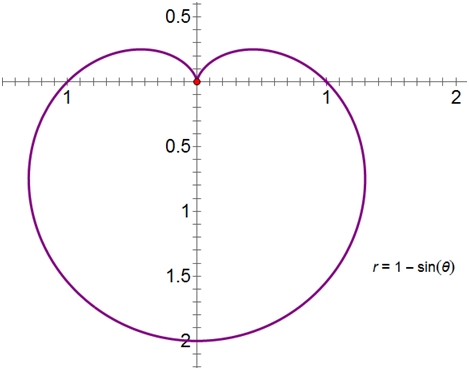
\includegraphics[scale=0.4]{r=1-sintheta.png}
			\caption{笛卡尔心形线~~~~~~}
		\end{figure}
		
	\end{center}
	
	
\end{frame}


\begin{frame}
	如果又有复数
	\[
	\beta=c+d {i}=|\beta|(\cos \psi+\operatorname{isin} \psi)
	\]
	那么
	\[
	\begin{aligned}
		\alpha \beta &=|\alpha||\beta|(\cos \varphi+i \operatorname{sin} \varphi)(\cos \psi+ i \operatorname{sin} \psi) \\
		&=|\alpha||\beta|(\cos \varphi \cos \psi-\sin \varphi \sin \psi)+(\sin \varphi \cos \psi+\cos \varphi \sin \psi) {i}) \\
		&=|\alpha||\beta|(\cos (\varphi+\psi)+i \operatorname{sin}(\varphi+\psi))
	\end{aligned}
	\]
	上式表示,两个复数相乘时,其模为这两个复数的模相乘,其辐角相 加(因为三角函数以 2 $\pi$ 为周期,故把相差 2 $\pi$ 的整数倍的角认为是相 同的).
\end{frame}

\begin{frame}{欧拉公式}
	令
	\[
	{e}^{{i} \varphi}=\cos \varphi+{i} \sin \varphi
	\]
	上式表示的复数模为 1,称为复数的\alert{欧拉公式}. 
	
	因而位于以坐标原点 O 为中心的单位圆上, 其辐角为 $\varphi$. 于是
	\[
	{e}^{{i} \varphi} {e}^{{i} \psi}={e}^{{i}(\varphi+\psi)}
	\]
	
	
	当$\varphi$为$\pi$时, $$ e^{i\pi }=-1$$
	将数学内4个极重要的数$e, i, \pi, -1 $连起来.
\end{frame}



\begin{frame}
	给定正整数 $n$,考查下列 $n$ 个复数
	\[
	{e}^{\frac{2 k \pi_{{i}}}{n}}=\cos \frac{2 k \pi}{n}+i\operatorname{sin} \frac{2 k \pi}{n}
	\]
	其中 $k=0,1,2, \cdots, n-1.$ 这 $n$ 个复数就是以坐标原点 $O$ 为中心的单 位圆的内接正 $n$ 边形的 $n$ 个顶点.
	于是
	\[
	\left({e}^{\frac{2 {k\pi i}}{n}}\right)^{n}=\left(\cos \frac{2 k \pi}{n}+i \operatorname{sin} \frac{2 k \pi}{n}\right)^{n}=\cos 2 k \pi+{i} \sin 2 k \pi=1
	\]
	因此,上面 $n$ 个复数 ${e}^{\frac{2 k \pi_{{i}}}{n}}=\cos \frac{2 k \pi}{n}+$ isin $\frac{2 k \pi}{n}$ 恰为 $n$ 次代数方程 $$x^{n}-1=0$$ 在复数系 $\mathbb{C}$ 内的 $n$ 个根,称为 $n$ 次单位根,它们是很有用的工
	具,在许多问题中都会用到.
\end{frame}


\end{document} 